\documentclass[11pt]{article}
\pdftrailerid{}
\usepackage{tikz}
\usepackage[a4paper,margin=24mm]{geometry}
\usepackage{amsmath,amssymb,amsthm,mathtools,microtype}
\usepackage{xcolor,xurl}
\usepackage[colorlinks=true,linkcolor=blue!50!black,urlcolor=blue!50!black,citecolor=blue!50!black]{hyperref}
\DeclareMathOperator{\spanof}{span}
\newtheorem{theorem}{Theorem}
\newtheorem{corollary}[theorem]{Corollary}
\newtheorem{lemma}[theorem]{Lemma}
\title{Weighted edge recoloring and 1-factorization across a cut}
\author{Juan Pablo Traverso Gianini\\\small Independent researcher, Santiago, Chile\\\small\href{mailto:jtraverso@gmail.com}{jtraverso@gmail.com}\quad\href{https://orcid.org/0009-0003-6068-4096}{ORCID 0009-0003-6068-4096}}
\date{Preprint 1.0 · November 24, 2026 · \mbox{\href{https://doi.org/10.5281/zenodo.24521352}{DOI 10.5281/zenodo.24521352}}}
\hypersetup{pdftitle={Weighted edge recoloring and 1-factorization across a cut},pdfauthor={Juan Pablo Traverso Gianini},pdfsubject={Preprint 1.0, DOI 10.5281/zenodo.24521352}}
\begin{document}
\maketitle

\begin{abstract}
To complete an internal edge coloring across a balanced cut, one must leave enough crossing copies for every color, especially at vertices with few distinct ordinary neighbors. We prove a weighted recoloring bound that preserves each prescribed class size. For equal sizes the scalar bound is sharp, and the optimal order for vector weights is the square root of the dimension of the span of the centered weights. Weighted Hall reserves then allow several exceptional vertices to be handled together. When the ordinary vertices are divided into blocks, the largest violation of a cut inequality gives the exact matching deficit under a width hypothesis. Each color attains its deficit using disjoint copies. We also give a 1-factorization criterion that combines the exceptional reserves with a hypergraph nibble and simultaneous repair in a spectral reserve. A regular grid family has \(\Theta(\sqrt N)\) distinct ordinary crossing neighbors per ordinary vertex and \(\Theta(N^{1/4})\) exceptions per side, where \(N\) is the number of ordinary vertices per side. A direct construction factors the family at an explicit threshold even though the rectangle criterion fails on its given cut for every admissible palette.
\end{abstract}

\section{Introduction}

The internal colorings and crossing matchings in the work of Shan~\cite{Shan} and Chen, McDonald and Shan~\cite{CMS} suggest the following approach for a regular multigraph of even order. We split its vertices into two equal parts, edge-color the two induced subgraphs, and complete each internal color to a perfect matching with crossing edges. Once this is done, the residual multigraph is regular and bipartite. Equalizing the sizes of the two internal classes of each color ensures that equal numbers of vertices on the two sides remain to be matched. Completion still depends on \emph{which} vertices remain, particularly when a vertex has few distinct crossing neighbors of large multiplicity.

For an exceptional vertex \(x\), an internal matching on the opposite side covers a set \(U\) of vertices. Exactly \(\sum_{v\in U}\mu(x,v)\) crossing copies from \(x\) end in \(U\), where \(\mu(x,v)\) denotes multiplicity. This count suggests assigning a weight to each vertex and asking how much weight each color covers. With several exceptional vertices, each \(v\) carries one coordinate for each \(x\). Changing a color class changes all these sums at once.

Our starting point is a scalar recoloring bound for prescribed class sizes. Section~\ref{sec:weights} gives the proof and a connected graph attaining the equal-size bound. Theorem~\ref{thm:balance} treats vector weights as well. Its bound depends on the dimension spanned by the centered weights, which can be much smaller than the number of exceptions. In Section~\ref{sec:cross} we use each coordinate to count the weight still available to one exceptional vertex. Assigning a crossing pair less weight than its multiplicity is useful when several exceptional vertices share a neighbor. The resulting inequalities give three sufficient conditions for completing the colors one at a time (Theorem~\ref{thm:factor}).

The same weighted reserves lead to two completion results. When ordinary vertices are divided into blocks, a color may have equal free counts on the two sides in total and unequal counts within a block. Theorem~\ref{thm:block-deficit} identifies the exact deficit from the eligible assignments of the exceptions. It also shows that all colors can attain their own deficits with disjoint crossing copies. Theorem~\ref{thm:hybrid-completion} addresses competition for copies across colors. After matching the exceptions, it uses one ordinary pool to build partial matchings for the whole palette and a second pool to repair them. The grid in Section~\ref{sec:sparse-reserve-example} illustrates the criterion. Its filler copies also give a direct construction with an explicit threshold, on a cut where the rectangle test fails for every admissible palette.

\subsection*{Relation to previous work}

Equitable edge colorings balance the numbers of edges in the color classes \cite{McDiarmid,CariolaroFu}. For bipartite graphs, the deduction in Section~\ref{sec:weights} gives an equitable-size scalar load bound from Nash-Williams's lemma on two laminar families~\cite{NashWilliams}. Theorem~\ref{thm:balance} prescribes every class size and allows odd cycles. Balister, Kostochka, Li and Schelp use alternating paths and a quadratic potential to balance the numbers of vertices with prescribed palettes \cite{BKLS}. Shioura and Yagiura balance edge counts globally and on parallel pairs \cite{SY}. Gajjala and Khan~\cite{GK} impose a capacity at each vertex in each color. The load considered here is the sum of the vertex weights over the entire matching.

The cut construction comes from the factorization arguments of Shan and of Chen, McDonald and Shan \cite{Shan,CMS}. Our hypotheses concern a specified cut and allow several exceptional vertices to share neighbors of large multiplicity. Section~\ref{sec:two-fifths} compares the degrees in one such family with those in earlier factorization results. In the spectral setting, Ferber and coauthors obtain an \(f\)-factor after bounded deletions under a hypothesis on the ambient graph \cite[Lemma~4.5]{FFMYZ}. The matrix in Theorem~\ref{thm:factor} measures the simple support between ordinary vertices on the prescribed cut. The block cut conditions use Gale's integral flow theorem~\cite{Gale}. Their role here is to determine how far weighted Hall completion can proceed after earlier colors have spent copies.

For simultaneous completion we use Keevash's nibble estimate, derived from work of Ehard, Glock and Joos~\cite{KeevashII,EGJ}. Broder, Frieze and Upfal~\cite{BFU} combine rapidly mixing walks and the Lov\'asz local lemma to route prescribed pairs in an expander. In Lemma~\ref{lem:spectral-repair}, the current matching determines the backward steps separately for each color. We count the use of each physical reserve copy across the whole palette and the use of each old matching edge within its color. Parallel edges in the host are treated as distinct copies.

\section{Recoloring with prescribed class sizes}\label{sec:weights}

All multigraphs are finite and loopless. We count parallel edges with multiplicity and regard their copies as distinct. For a proper edge coloring \(M_1,\ldots,M_k\) and a vertex weight function \(w\), write
\[
  m_i=|M_i|,\qquad W_i=\sum_{uv\in M_i}\bigl(w(u)+w(v)\bigr).
\]
Since each \(M_i\) is a matching, \(W_i\) is the sum of the weights of the vertices it covers.

\begin{theorem}\label{thm:balance}
Let \(G\) admit a proper edge coloring with class sizes \(m_1,\ldots,m_k\). Let \(w\) take values in a finite-dimensional real Euclidean space. Fix \(c\) and \(R\ge0\) with \(\|w(v)-c\|_2\le R\) for all \(v\), and put \(s=\dim\spanof\{w(v)-c:v\in V(G)\}\). There is a proper edge coloring in which color \(i\) still has size \(m_i\) for every \(i\) and, for all \(i,j\),
\[
  \|(W_i-2m_i c)-(W_j-2m_j c)\|_2
  \le 2R\,\psi_s(|m_i-m_j|),
\]
where
\[
 \psi_s(d)=
 \begin{cases}
   0 & s=0,\\
   2 & s=1,\ d=0,\\
   d & s=1,\ d>0,\\
   \sqrt{d^2+4s} & s\ge2.
 \end{cases}
\]
\end{theorem}

\begin{proof}
Write \(z(v)=w(v)-c\) and \(Z_i=W_i-2m_i c\). The statement is immediate for \(s=0\). In the finite set of colorings with the given class sizes, minimize \(\sum_i\|Z_i\|_2^2\). Fix distinct color labels \(i,j\), with \(d=m_i-m_j\ge0\), and consider the components containing edges in the subgraph of those two colors. These are alternating paths and even cycles, with two parallel edges allowed as a cycle of length two. Both colors cover each internal vertex of a path and each vertex of a cycle. Thus a cycle contributes zero to \(Z_i-Z_j\). An even path with end vertices \(u,v\) contributes a signed copy of \(z(u)-z(v)\), while an odd path contributes a signed copy of \(z(u)+z(v)\). Every sign is available by interchanging the two colors on the component. An odd path contributes the same sign to \(m_i-m_j\).

Let \(r\) be the number of odd paths, so that \(r\ge d\) and \(r\equiv d\pmod 2\). Choose \(d\) odd paths with sign \(+1\), and pair the others with opposite signs in each pair. These choices preserve the difference between the two class sizes. Their sum is fixed as well, so both colors retain their prescribed sizes. The load difference takes the form
\[
  u_0+\sum_{\ell=1}^q \varepsilon_\ell v_\ell,\qquad
  \|u_0\|_2\le 2Rd,\qquad \|v_\ell\|_2\le4R,
\]
where each independent sign represents one even path or one pair of odd paths. An even path has \(\|v_\ell\|_2\le2R\).

When \(s=1\), we identify the span with the real line. For \(d=0\) any pairing of the odd paths suffices. For \(d>0\) we group the odd paths according to whether their endpoint sums are negative or nonnegative. We first set aside one path from each group of odd size. The number set aside has the parity of \(d\) and is at most \(d\): it is at most two, and when \(d=1\) it must be one. Both groups now have even size. Since \(r\ge d\), we can set aside additional pairs until we have \(d\) paths to orient positively. All remaining pairs can be formed within groups. For this within-group pairing the sums differ by at most \(2R\), since the sums in a group lie in an interval of length \(2R\). For \(d=0\) the unrestricted pairing instead gives the bound \(4R\). Starting at \(u_0\), we choose signs successively to oppose the current sum. The final absolute value is at most \(\max(|u_0|,\max_\ell |v_\ell|)\), with the latter maximum zero if there are no signs to choose. The desired bounds are \(4R\) for \(d=0\) and \(2Rd\) for \(d>0\).

For equal class sizes the remaining choice of signs is the classical Euclidean balancing problem studied by Spencer~\cite{Spencer}. We also need to allow the fixed displacement \(u_0\) when the sizes differ. The following reduction and rounding argument follows the method of Ambrus and Bozzai~\cite[Section~2 and Proposition~3.1]{AB}. Here the vectors to be signed come from swaps that preserve both class sizes. Minimizing the energy over colorings will make the bound hold for every pair in the same coloring.

For \(s\ge2\), we start with coefficients \(x_\ell=0\) in the cube \([-1,1]^q\), with \(\sum_\ell x_\ell v_\ell=0\). If there are more than \(s\) interior coordinates, a nonzero dependence among the corresponding \(v_\ell\) gives a direction preserving this equation. Choosing the direction on the interior coordinates keeps every boundary coefficient fixed. Moving to the first new boundary point preserves the vector sum and fixes at least one more coefficient. Each step reduces the number of interior coordinates, so iteration leaves at most \(s\) of them.

We round the remaining coefficients one at a time. For a partial sum \(u\) and one contribution \(xv\), the convex combination of \(\|u+v\|_2^2\) and \(\|u-v\|_2^2\) with coefficients \((1+x)/2,(1-x)/2\) equals \(\|u+xv\|_2^2+(1-x^2)\|v\|_2^2\). At least one sign gives squared norm at most this average. The cumulative extra squared norm is at most the sum of these costs. The initial sum is \(u_0\), so the resulting squared norm is at most
\[
  \|u_0\|_2^2+\sum_\ell(1-x_\ell^2)\|v_\ell\|_2^2
  \le 4R^2(d^2+4s).
\]

The sum \(Z_i+Z_j\) and the loads of all other colors stay fixed under these changes. The identity
\[
  2\bigl(\|Z_i\|_2^2+\|Z_j\|_2^2\bigr)
    =\|Z_i+Z_j\|_2^2+\|Z_i-Z_j\|_2^2
\]
would give a strict improvement of the minimum if the original difference exceeded the asserted bound. Hence the minimizing coloring satisfies all the bounds.
\end{proof}

\begin{corollary}[Sharp scalar bounds]\label{cor:scalar}
If \(w:V(G)\to[L,U]\), one can preserve the prescribed sizes and achieve, simultaneously for all \(i,j\),
\[
\begin{aligned}
 |W_i-W_j|&\le2(U-L) &&\text{if }m_i=m_j,\\
 2L(m_i-m_j)&\le W_i-W_j\le2U(m_i-m_j)
       &&\text{if }m_i>m_j.
\end{aligned}
\]
\end{corollary}

\begin{proof}
With \(c=(L+U)/2\) and \(R=(U-L)/2\), Theorem~\ref{thm:balance} bounds the centered difference. Adding \(2(m_i-m_j)c\) gives the stated endpoints.
\end{proof}

For comparison, suppose the graph is bipartite and the desired sizes are equitable. On each side order the vertices by weight. The stars and the unions of stars over initial segments form a laminar family of edge sets, including the full edge set. Nash-Williams's lemma \cite{NashWilliams} splits off one color at a time with the floor or ceiling of the proportional size in each set. The final counts differ by at most one in each set. The star constraints give a proper coloring when the number of colors is at least the maximum degree. For two classes of equal size, summation by parts then bounds their load difference by the sum of the two weight ranges, one from each side.

The constant \(2\) in the equal-size bound is attained in a connected simple graph. The example is a triangle \(abc\) with three additional edges \(ad,de,bf\), with weight \(U\) at \(c,f\) and weight \(L\) at the remaining four vertices. In any proper coloring with three classes of size two, we may relabel the colors so that \(ab,ac,bc\) have colors \(1,2,3\). The edges \(ad,bf\) must have colors \(3,2\), and the class sizes force color \(1\) on \(de\). The resulting loads are \(4L,2L+2U,3L+U\).

The Euclidean dependence on \(s\) has optimal order. For even \(s\), give both endpoints of the \(j\)-th edge of a matching the weight \(Re_j\), \(1\le j\le s\), with \(e_j\) the coordinate vectors and \(R>0\). In every split into two equal color classes, the discrepancy has norm \(2R\sqrt{s}\).

\section{From recoloring to crossing matchings}\label{sec:cross}

Let \(M\) be a \(D\)-regular multigraph with a partition \(A,B\), where \(|A|=|B|=m\). Let \(X\subseteq A\) and \(Y\subseteq B\) be the exceptional vertices and set \(A_0=A\setminus X\) and \(B_0=B\setminus Y\). For \(u,v\in V(M)\), let \(\mu(u,v)\) be the number of copies of \(uv\). By the support of the crossing graph we mean its simple graph of distinct crossing neighbors.

Suppose \(1\le k<D\) and \(M[A],M[B]\) each admit a proper edge coloring with \(k\) colors. In either coloring, if two classes differ in size by at least two, an odd alternating path with one more edge of the larger class exists. Switching its colors decreases the sum of squared class sizes. Repeating this step gives equitable colorings on both sides \cite{McDiarmid,CariolaroFu}. If \(e_A,e_B\) count internal edges and \(e_\times\) counts crossing copies, regularity gives
\[
 2e_A+e_\times=Dm=2e_B+e_\times.
\]
Thus the equitable classes have the same multiset of sizes on each side, and we can pair classes of equal size. Write \(a_i\) for the resulting common sizes, and put
\[
 a=\max_i a_i=\left\lceil e(M[A])/k\right\rceil,\qquad
 d_*=\max_{i,j}|a_i-a_j|\in\{0,1\}.
\]
Let \(\sigma_A,\sigma_B\) be upper bounds on the internal degrees of ordinary vertices in their respective parts. Let \(\delta_A,\delta_B\) be lower bounds on the number of distinct crossing neighbors in the opposite ordinary part, for ordinary vertices on each side.

For \(x\in X\), choose a nonnegative charge \(\eta_x\) for one spent copy. Choose pair weights \(w_{xv}\) satisfying
\[
 0\le w_{xv}\le \eta_x\mu(x,v)\quad (v\in B_0),\qquad
 \sum_{x\in X}w_{xv}\le C_X\quad(v\in B_0),
\]
where \(C_X>0\). Extend each row by zero at the vertices of \(Y\) and put \(T_x=\sum_{v\in B_0}w_{xv}\). The column of weights at \(v\in B\) is denoted by \(w_X(v)\). The discrepancy estimate depends on whether the weights have a scalar or a vector representation.
\begin{itemize}
\item If \(w_{xv}=t_v u_x\) for the full part \(B\), with \(0\le t_v\le R\) and \(u_x\ge0\), set \(H_x=2R u_x\).
\item If \(w_{xv}=c_x+\langle u_x,z_v\rangle\) on the vertices nonisolated in \(M[B]\), where \(z_v\in\mathbb R^s\), \(\|z_v\|_2\le R\) and \(\|u_x\|_2\le1\), one may use
\[
 H_x=2R\|u_x\|_2\sqrt{d_*^2+4s}+2|c_x|d_* .
\]
\end{itemize}
In the vector case one can use orthonormal coordinates on the span of the centered profiles. At a vertex isolated in the internal graph the choice of \(z_v\) has no effect on any internal load. The data for \(Y\) are defined symmetrically. The case \(w_{xv}=\eta_x\mu(x,v)\) is the usual fixed rescaling of each row.

For a row on the left put
\[
 I_x=\sum_{v\in B_0}\deg_{M[B]}(v)w_{xv},
\]
and define \(I_y\) using the internal degrees on the left. Thus \(I_x\le\sigma_B T_x\).

\begin{lemma}[Available crossing weight]\label{lem:available}
There is a proper coloring of all internal edges, with sizes \(a_i\) on both sides, such that the following holds for every color \(i\). After discarding the vertices covered by its internal edges, and after spending at most \(p\) copies of crossing edges per vertex, each surviving \(x\in X\) has weight at least
\[
 T_x-I_x/k-\frac{k-1}{k}H_x-p\eta_x
\]
in residual certificate weight on edges to the surviving vertices of \(B_0\). The symmetric estimate holds for \(y\in Y\).
\end{lemma}

\begin{proof}
In the scalar case apply Corollary~\ref{cor:scalar} to \(t_v\). Equitable sizes give a scalar difference of magnitude at most \(2R\). Scaling by \(u_x\) proves the bound for every row in a single coloring. In the vector case apply Theorem~\ref{thm:balance} to \(z_v\), using the bound with \(\sqrt{d_*^2+4s}\), which also dominates the scalar clause. The \(x\)-load equals the projection of the \(z_v\)-load plus \(2c_x a_i\). Cauchy--Schwarz bounds the projection, and the difference of the affine terms is at most \(2|c_x|d_*\) in magnitude. In each case color \(i\) still has exactly \(a_i\) edges.

Let \(W_{x,i}\) be the load of color \(i\) in row \(x\). Each ordinary vertex \(v\) is covered by exactly \(\deg_{M[B]}(v)\) colors. Hence
\[
 \frac1k\sum_j W_{x,j}=I_x/k,\qquad
 W_{x,i}-\frac1k\sum_jW_{x,j}
       =\frac1k\sum_{j\ne i}(W_{x,i}-W_{x,j})
       \le\frac{k-1}{k}H_x.
\]
The vertices covered internally account for weight \(W_{x,i}\). If \(s_{xv}\) copies of a crossing pair were spent, use the residual certificate \(w'_{xv}=(w_{xv}-\eta_x s_{xv})_+\). This is zero when every copy is gone. On the set \(U\) of free ordinary vertices we therefore have
\[
 \sum_{v\in U} w'_{xv}
 \ge \sum_{v\in U} w_{xv}-\eta_x\sum_{v\in U}s_{xv}
 \ge T_x-W_{x,i}-p\eta_x.
\]
Substitution of the preceding bound on \(W_{x,i}\) gives the assertion. The estimates on the other side follow by applying the same argument to \(w_Y\) in \(M[A]\). The sizes in both parts remain \(a_i\) for each \(i\).
\end{proof}

\begin{theorem}[Factorization across a cut]\label{thm:factor}
With the notation above, suppose the exceptional rows satisfy
\begin{align}
  T_x-I_x/k&\ge C_X+\frac{k-1}{k}H_x+(k-1)\eta_x
      &&(x\in X),\label{eq:rowx}\\
  T_y-I_y/k&\ge C_Y+\frac{k-1}{k}H_y+(k-1)\eta_y
      &&(y\in Y).\label{eq:rowy}
\end{align}
Suppose also that one of the following conditions holds.
\begin{enumerate}
\item The ordinary crossing degrees satisfy
\[
  \delta_A+\delta_B\ge m+2a+2(k-1).
  \tag{D}\label{eq:dense}
\]
\item Put \(\ell=2a+\max(|X|,|Y|)\). There are positive integers \(\rho,\tau\) such that
\[
 \rho\ge\ell,\qquad \rho\ge k,\qquad
 \min(\delta_A,\delta_B)\ge\tau+\ell+k-1,
 \tag{R}\label{eq:robust}
\]
and for every \(S\subseteq A_0\) with \(\tau\le |S|\le |A_0|-\tau\), there are at least \(|S|+\rho\) vertices in \(B_0\) having at least \(\rho\) neighbors in \(S\) in the crossing support.
\item The exceptional sets have the same size \(r\). On the \(N=m-r\) ordinary vertices per side, the simple crossing support is \(d\)-regular with \(1\le d\le N\). Let \(\lambda\) be the operator norm of its biadjacency matrix on vectors perpendicular to the constants, equivalently its second singular value (zero on the zero-dimensional subspace). Assume
\[
 \lambda\le 3d/4,\qquad 2a+r+k-1\le d/8 .
 \tag{S}\label{eq:spectral}
\]
\end{enumerate}
Then \(M\) has a 1-factorization. More generally, it suffices that for each pair of nonempty sets \(S\subseteq A_0\), \(T\subseteq B_0\) with
\[
 |S|+|T|>m-2a-|X|-|Y|
\]
there is a vertex in \(S\cup T\) incident with at least \(k\) crossing copies between \(S\) and \(T\).
\end{theorem}

\begin{proof}
We start with the internal coloring supplied by Lemma~\ref{lem:available} and complete its classes in any order. When we reach color \(i\), let \(p\le k-1\) be the number of classes completed, and keep only available crossing edges on the \(m_i'=m-2a_i\) uncovered vertices on each side. Previous completions spent at most \(p\) copies at each vertex.

Each surviving \(x\in X\) has weighted degree at least \(C_X\) toward surviving ordinary vertices. In every column, the total weight from all such \(x\) is at most \(C_X\). For any subset \(Q\) of these exceptional vertices, count the available weight between \(Q\) and its ordinary neighborhood \(N_0(Q)\) to obtain
\[
   C_X|Q|\le \sum_{x\in Q}\sum_{v\in N_0(Q)}
             w'_{xv}\le C_X|N_0(Q)|.
\]
Every positive residual weight has an available copy. Hall's condition toward ordinary vertices follows. The same argument applies to the surviving exceptional vertices of \(Y\).

Suppose that a set \(Q\) of free vertices on the left has fewer neighbors than members. Let \(P\) be the free right vertices outside its residual neighborhood. Then \(|Q|+|P|>m_i'\), and the neighbors of \(P\) all lie outside \(Q\). Exceptional Hall on both sides ensures that \(S=Q\cap A_0\) and \(T=P\cap B_0\) are nonempty. Their sizes satisfy \(|S|+|T|>m-2a-|X|-|Y|\).

Every original crossing copy between \(S\) and \(T\) has been spent, since both endpoints remain free and no residual edge joins them. This proves the general assertion: a vertex with \(k\) copies across the pair would have spent more than the \(p\le k-1\) copies allowed so far. It is also enough to find \(k\) distinct neighbors of a vertex across the pair. For this it suffices to have more than \((k-1)\min(|S|,|T|)\) support edges, by averaging over the smaller side.

Write \(s=|S|\), \(t=|T|\). Under~\eqref{eq:dense}, if every vertex has at most \(k-1\) neighbors across the pair, then
\[
 \delta_A+\delta_B\le |B_0|-t+|A_0|-s+2(k-1)<m+2a+2(k-1).
\]
This contradicts the degree condition.

For the bipartite robust neighborhood of K\"uhn, Lo, Osthus and Staden~\cite{KLOS}, apply~\eqref{eq:robust} as follows. If \(s\le\tau\), then \(|B_0|-t<s+2a+|X|\). Each vertex of \(S\) therefore has at least \(k\) neighbors in \(T\), by the degree bound. If \(s>|A_0|-\tau\), the degree bound gives at least \(k\) neighbors in \(S\) for each vertex of \(T\). In the remaining range the robust neighborhood of \(S\) contains at least \(s+\rho\) vertices. The inequality \(|B_0|-t<s+2a+|X|\le s+\rho\) puts a robust neighbor in \(T\). It has at least \(\rho\ge k\) neighbors in \(S\).

For~\eqref{eq:spectral}, suppose that the original support has at most \(k-1\) neighbors across the pair at every vertex. Put \(b=k-1\) and \(h=2a+r\). Regularity of the support gives \(d\le N-t+b\) and \(d\le N-s+b\). Since \(s+t>N-h\), we obtain
\[
 \min(s,t)>d-h-b\ge 7d/8,\qquad
 \max(s,t)>\frac{(7+u)N}{16},\qquad u=8b/d.
\]
The second inequality uses \(h\le (1-u)d/8\) and \(d\le N\).

Let \(e\) be the number of support edges between \(S\) and \(T\). The assumption on the degrees gives \(e\le b\min(s,t)\). For the lower bound, center the indicators of \(S\) and \(T\) separately by subtracting \(s/N\) and \(t/N\). Regularity cancels the mixed terms with a constant vector. The mixing bound~\cite{Haemers} gives
\[
 e\;\ge\;\frac{dst}{N}
 \left(1-\frac{\lambda}{d}\sqrt{\frac{(N-s)(N-t)}{st}}\right).
\]
The ratio in the square root satisfies
\[
 \frac{(N-s)(N-t)}{st}
 =1+\frac{N(N-s-t)}{st}
 \le \frac{65-9u}{7(7+u)} .
\]
Here we used \(N-s-t<h\) and the bounds on the smaller and larger sets. The normalized upper bound on \(e\) is \(bN/(d\max(s,t))\le 2u/(7+u)\), strictly if \(u>0\). The normalized lower bound is at least
\[
 1-\frac34\sqrt{\frac{65-9u}{7(7+u)}}\ge \frac{2u}{7+u}.
\]
To see the last inequality, square the equivalent inequality between nonnegative quantities. The difference after clearing denominators is
\[
 112(7-u)^2-9(7+u)(65-9u)=(1-u)(1393-193u).
\]
It is nonnegative for \(0\le u\le1\) and positive at \(u=0\). This contradicts the upper bound on \(e\).

In each case, the internal edges and the crossing matching of color \(i\) form a 1-factor. The argument uses only available copies, so we can repeat it for every internal color. The residual multigraph is \((D-k)\)-regular and bipartite. Counting degrees gives Hall's condition in every positive-degree regular bipartite multigraph, so repeated removal of perfect matchings factors the residue.
\end{proof}

The row and column constraints are closely related to capacitated transportation, for which Gale's feasibility theorem gives cut certificates \cite{Gale}. The recoloring ensures that each color leaves the required row totals available.

\section{Examples}\label{sec:examples}

In each example the internal ordinary graph is a disjoint union of copies of \(K_{2,2}\), one on each group of four ordinary vertices. The exceptional vertices are isolated in the internal graphs. The internal degree of an ordinary vertex is two. Thus any palette with at least two colors is available, with \(N\) internal edges on each side when there are \(N\) ordinary vertices per side.

\subsection{A shared heavy neighbor}

Each side has \(N=4r\) ordinary vertices, with \(r\ge6\), and two exceptional vertices. Each exceptional vertex sends \(N\) copies to a common distinguished ordinary vertex on the opposite side and one copy to each of \(N/2\) further shared vertices. The ordinary parts span a complete bipartite support. On each pair of corresponding ordinary vertices we add \(2N\) copies less the incidence it receives from exceptional vertices. Between corresponding exceptional vertices we place \(D-3N/2\) copies, where \(D=3N+2\). This gives degree \(D\) everywhere.

Here \(k=4\) and \(a=N/4\). The degree condition~\eqref{eq:dense} holds. For \(w_{xv}=\min(1,\mu(x,v))\) the rows are identical and \(T_x=N/2+1\), \(C_X=2\), \(H_x=2\), \(\eta_x=1\). The available weight in the row inequality is \((N/2+1)(1-2/4)\). Its required weight is \(2+(3/4)2+3=13/2\), so \(N\ge24\) suffices. The opposite side has the same weights and the same degrees.

The same cut fails every fixed row rescaling of the original multiplicities. Indeed, writing \(D_x=\sum_{v\in B_0}\mu(x,v)\), the necessary inequalities \(\eta_xD_x\ge C_X>0\) and \(\sum_x\eta_x\mu(x,v)\le C_X\) imply \(\sum_x\mu(x,v)/D_x\le1\). At the distinguished column it is \(2N/(3N/2)=4/3\).

\subsection{A common baseline in a growing family}

Each side has \(r\ge6\) exceptional vertices and \(N=4r\) ordinary vertices in groups of four. The four ordinary vertices in group \(j\) have \(q+\mathbf1_{x=j}\) copies to the opposite exceptional vertex \(x\), for an integer \(q\ge2\). Every exceptional vertex has degree \(D=Nq+4\). The ordinary crossing multigraph is complete simple support plus equal additional multiplicity on corresponding pairs to bring its degree to \(3rq+1\). The graph is \(D\)-regular since the remaining degrees at an ordinary vertex are \(rq+1\) and \(2\).

For \(k=4\) and \(a=N/4\), the two ordinary degrees sum to \(2N\), whereas the right side of~\eqref{eq:dense} is \(N+r+N/2+6\le2N\). With unit charges and the actual multiplicities as weights, \(T_x=Nq+4\), \(C_X=rq+1\). Take \(z_v=e_j\) at an ordinary vertex in group \(j\), \(u_x=e_x\), and \(c_x=q\). The equitable sizes are equal, so the shift term vanishes. The allowance \(H_x=2r\) is sufficient since \(4\sqrt r\le2r\). Subtracting the required weight from the available weight gives
\[
 \tfrac12(4rq+4)-(rq+1)-\tfrac34(2r)-3
 =rq-\tfrac32r-2\ge \tfrac12r-2>0 .
\]

For comparison, the uncentered columns have full rank \(r\). If coefficients \(\alpha_j\) give a dependence, the equations are \(\alpha_x+q\sum_j\alpha_j=0\) for every \(x\). Summing shows \(\sum_j\alpha_j=0\), hence each coefficient is zero. Fixed positive scaling of each row preserves the rank. If \(\eta_{\min}\) is the smallest scale, the scaled radius is at least \(q\sqrt r\,\eta_{\min}\). Using the Euclidean norm of the scaled incidence columns, the uncentered estimate would charge at least \(3qr\,\eta_{\min}\) for discrepancy alone in that row, exceeding \((Nq+4)\eta_{\min}/2\), its available budget before deductions.

This comparison concerns the Euclidean estimate on the multiplicity columns. The same graph also admits a scalar certificate without centering if we change the weights. Every exceptional--ordinary pair has positive multiplicity, so its indicator is one. With \(T_x=4r\), \(C_X=r\), \(\eta_x=1\) and \(H_x=2\), the row inequality becomes \(2r\ge r+9/2\), which holds for \(r\ge6\).

One can also center the multiplicity columns at \((q+1/r)\mathbf1\). The centered vectors \(e_j-\mathbf1/r\) span the sum-zero space of dimension \(r-1\), with radius \(\sqrt{1-1/r}\). Projecting each coordinate onto this space gives the same norm \(\sqrt{1-1/r}\) for the corresponding row. With equal sizes the row allowance becomes \(4(r-1)^{3/2}/r\).

\subsection{Robust completion at two fifths of the ordinary part}\label{sec:two-fifths}

Let \(b\) be a positive multiple of \(400\), let \(g=b-2\), and put \(r=5g\), \(N=rb\). On each side there are \(r\) exceptional vertices and \(N\) ordinary vertices. The ordinary vertices form \(r\) groups of size \(b\). Every ordinary vertex in group \(j\) sends \(g+1\) copies to each of the opposite exceptional vertices \(j,j+1\), with indices interpreted cyclically. On each ordinary side a second partition gives five equal blocks of size \(B=N/5\). Across the cut we join blocks with \(i+j\in\{0,1\}\) modulo five by complete simple bipartite support. The block graph is a bipartite ten-cycle. There are no edges between exceptional vertices. Every exceptional vertex has degree \(D=2b(g+1)\). The ordinary degree is \(2+2(g+1)+2B=D\).

With \(k=100\) colors we have \(a=N/100\). The incidence weights are the indicators of a positive exceptional multiplicity, and the charges are one. The column weight is \(2\), each row has total \(2b\), and the column vectors have norm at most \(2\). With equal sizes and \(s=r\), the allowance \(H_x=b\) suffices because \(b^2\ge64r\). The row inequality holds since \(98(2b)/100\ge 2+99+99b/100\).

Take \(\rho=N/40\), \(\tau=5\rho\). For a set \(S\) with \(\tau\le|S|\le N-\tau\), let \(J\) be the block indices containing at least \(\rho\) vertices of \(S\). At least one block lies in \(J\). If \(J\) is the full set, all \(N\) right vertices are robust neighbors, and \(N\ge |S|+\tau\ge |S|+\rho\). For \(1\le |J|<5\), the block graph gives at least \(|J|+1\) right blocks of robust neighbors. Meanwhile \(|S|\le |J|B+5\rho\). Their difference is at least \(\rho\) because \(6\rho\le B\). To check the degree bound, note that \(r=N/b\) and \(b\ge400\), so
\[
 (2a+r)/\rho=40(2/100+1/b)\le 9/10.
\]
Also \(\rho=rb/40\ge100=k\). Hence \(\tau+2a+r+k-1\le7\rho\le 2B\), as required. The ordinary crossing degree is \(2N/5\), so the dense degree condition fails on this cut.

This family also illustrates the role of the exceptional sets in earlier factorization theorems. Deleting one vertex still leaves several pairs of multiplicity greater than one, outside the near-star hypotheses of Shan \cite[Theorem~3.1]{Shan}. The degree and maximum multiplicity fail the bound \(D\ge\mu_{\max}(n/2+18)\) of Plantholt and Shan \cite[Theorem~1.6]{PlantholtShan}. In the small-parameter regime of Chen, McDonald and Shan \cite[Theorem~4.2]{CMS}, the simple degree bound on the third and subsequent vertices in the exceptional ordering is linear in \(D\). Here each of the \(r=5(b-2)\) exceptions on a side has only \(2b\) distinct neighbors while \(D=2b(b-1)\).

\subsection{A sparse ordinary crossing graph}\label{sec:grid}

Let \(q\ge46\) be an integer. Each side contains a \(q\)-by-\(q\) array with 256 ordinary vertices in each cell and one exceptional vertex per row. Thus \(N=256q^2\) and \(r=q\). Two opposite cells are joined completely when they share a row or a column, including the corresponding cell. The simple ordinary crossing degree is
\[
 d=256(2q-1)=32\sqrt N-256 .
\]
Each ordinary vertex sends \(q\) copies to the opposite exceptional vertex in its row. Inside each cell are 64 disjoint copies of \(K_{2,2}\). The exceptional vertices are internally isolated. An exceptional vertex now has degree \(256q\cdot q=N\), while an ordinary vertex has degree \(d+q+2\). We add \(N-d-q-2\ge0\) parallel copies on each pair of corresponding ordinary vertices. This makes the multigraph \(N\)-regular and preserves the crossing support.

To compute the singular values, let \(J_n\) denote the all-ones matrix and \(I_n\) the identity. The matrix on cell indices is
\[
 I_q\otimes J_q+J_q\otimes I_q-I_q\otimes I_q .
\]
It has eigenvalue \(2q-1\) on constants, \(q-1\) on functions of a single coordinate of mean zero, and \(-1\) on the tensor product of the two mean-zero spaces. These subspaces span the cell functions. Replacing each entry by that entry times \(J_{256}\) multiplies these eigenvalues by 256 and adds zeros. The matrix is symmetric, so \(\lambda=256(q-1)\le d/2\).

There are \(N\) internal edges per side. With \(k=16q\) we get \(a=N/k=16q\) and \(d_*=0\). The ordinary weights for row \(x\) are its incidence indicators, with charge one. Each column has a single one, each row has total \(256q\), and \(\sigma_A=\sigma_B=2\). The profiles are coordinate vectors, so \(R=1\), \(s=q\) and \(H_x=4\sqrt q\). In the row inequality the available and required weights satisfy
\[
 T_x(1-2/k)=256q-32,\qquad
 1+(k-1)H_x/k+(k-1)\le16q+4\sqrt q\le256q-32 .
\]
Also \(2a+r+k-1=49q-1\le64q-32=d/8\). Theorem~\ref{thm:factor} gives a 1-factorization. The ordinary crossing density \(d/N=(2q-1)/q^2\) tends to zero.

Fix this cut and its exceptional sets, and now allow any admissible palette \(k\). Condition~\eqref{eq:dense} already fails because \(2d<N+q=m\). For~\eqref{eq:robust}, suppose that thresholds \(\rho,\tau\) work. Since \(ak\ge N\),
\[
 \rho\ge\max(2a,k)\ge\sqrt{2ak}\ge\sqrt{2N}>1024 .
\]
The degree condition gives \(\tau\le d\), and \(2d\le N\), so a set of size exactly \(\tau\) lies in the range tested for expansion. Number the rows and columns modulo \(q\). The two diagonals \(j=i\) and \(j=i+1\) contain \(512q>d\) vertices in total. Choose \(\tau\) of them on the left. Each opposite cell meets them through at most two cells in its row and two in its column. Every right ordinary vertex therefore sees at most \(4\cdot256=1024\) selected vertices. The robust neighborhood is empty, contradicting its required size \(\tau+\rho\). This proves the separation for every palette on the specified cut.

\subsection{A rectangular grid}

The rectangular version has \(2q\) rows and \(q\) columns with \(q\ge49\). It retains the 256 ordinary vertices per cell and one exceptional vertex per row. The ordinary crossing support has degree \(d=256(3q-1)\) on \(N=512q^2\) vertices per side. The row and column functions of mean zero now have eigenvalues \(256(q-1)\) and \(256(2q-1)\), respectively. The constant and tensor-product spaces give \(d\) and \(-256\), and functions summing to zero in each cell give zero. Thus the ratio \((2q-1)/(3q-1)\) lies between \(1/2\) and \(3/4\).

We place \(2q\) copies between each ordinary vertex and the opposite exceptional vertex in its row. We retain the internal graphs and add copies between corresponding ordinary vertices to make every degree \(N\). For \(k=32q\) and \(a=16q\), the indicator rows have available weight \(256q-16\) before the discrepancy and spending deductions. The required weight is at most \(32q+4\sqrt{2q}\), and the spectral budget is \(66q-1\le d/8\). This gives a 1-factorization.

The fixed cut fails~\eqref{eq:dense} because \(2d<N+2q\). To test~\eqref{eq:robust}, use columns \(i\) and \(i+1\) modulo \(q\) in row \(i\). There are \(1024q\ge d\) ordinary vertices in these cells, so they contain a set of size \(\tau\) in the expansion window. As Figure~\ref{fig:rectangle} illustrates, an opposite vertex sees at most two selected cells in its row and four in its column. Its degree into the set is at most 1536, whereas \(\rho\ge\sqrt{2N}=32q>1536\) for every admissible palette. The support density is \((3q-1)/(2q^2)\). The multigraphs themselves remain \(N\)-regular.

\begin{figure}[ht]
\centering
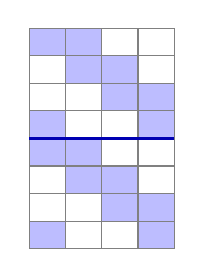
\begin{tikzpicture}[x=.46cm,y=.35cm]
\foreach \i in {0,...,7} {
  \foreach \j in {0,...,3} {
    \pgfmathtruncatemacro{\firstcol}{mod(\i,4)}
    \pgfmathtruncatemacro{\nextcol}{mod(\i+1,4)}
    \ifnum\j=\firstcol \fill[blue!26] (\j,-\i) rectangle +(1,-1); \fi
    \ifnum\j=\nextcol \fill[blue!26] (\j,-\i) rectangle +(1,-1); \fi
    \draw[gray] (\j,-\i) rectangle +(1,-1);
  }
}
\draw[very thick,blue!70!black] (0,-4) -- (4,-4);
\end{tikzpicture}
\caption{The two choices of column in each row of the rectangle, shown with four columns. Each row contains two selected cells, and each column contains four. The heavy line separates the two copies of the cyclic pattern.}\label{fig:rectangle}
\end{figure}

\section{Exceptional assignments and exact block deficits}\label{sec:block-routing}

The ordinary vertices of a cut can be divided into corresponding blocks. Even if the two sides have the same total number of free vertices in a given color, their free counts can differ within a block. Assigning an exceptional vertex to a block uses one ordinary vertex on the opposite side and changes that difference by one.

Fix a color. Write \(u_j,v_j\) for the ordinary free counts on the left and right of block \(j\) and put \(\delta_j=u_j-v_j\). Let \(X,Y\) be the free exceptional sets on the two sides. Each exception has a set of eligible blocks. If \(p^A_j,p^B_j\) count the left and right exceptions assigned to \(j\), the remaining ordinary sides there have sizes \(u_j-p^B_j\) and \(v_j-p^A_j\). They are equal exactly when
\[
 p^B_j-p^A_j=\delta_j.
\]
The total balance of free vertices gives \(\sum_j\delta_j=|Y|-|X|\). For a set \(S\) of blocks, let \(L(S)\) count the left exceptions whose eligible blocks all lie in \(S\), and let \(R(S)\) count the right exceptions with an eligible block in \(S\). We write \(\delta(S)=\sum_{j\in S}\delta_j\).

For example, suppose there are two blocks with \(\delta_1=1\) and \(\delta_2=-1\). The width assumptions below can be met by taking \((u_1,v_1)=(\theta+2,\theta+1)\) and \((u_2,v_2)=(\theta+1,\theta+2)\), with threshold \(\theta\) in both blocks. If the left exception can use only block~1 and the right exception only block~2, then \(L(\{1\})=1\) and \(R(\{1\})=0\). The first singleton cut has gap \(1-0+1=2\). Allowing the right exception to use both blocks reduces the largest gap to \(1\). Allowing the left exception to use both blocks reduces it to \(0\), since we can now send the left exception to block~2 and the right exception to block~1. Theorem~\ref{thm:block-deficit} turns these cut gaps into exact matching deficits.

\begin{lemma}[Assignment across blocks]\label{lem:block-assignment}
Assume total balance. There is an eligible assignment with \(p^B_j-p^A_j=\delta_j\) at every block if and only if
\[
 \delta(S)\le R(S)-L(S)
 \qquad\text{for every set \(S\) of blocks.}
 \tag{A}\label{eq:block-assignment}
\]
If each right count must also satisfy \(p^B_j\le c_j\), for given nonnegative integers \(c_j\), the necessary and sufficient condition is
\[
 \delta(S)\le R(T)-L(S)+\sum_{j\in S\setminus T}c_j
 \qquad\text{for every two sets \(S,T\) of blocks.}
 \tag{C}\label{eq:block-capacity}
\]
\end{lemma}

\begin{proof}
For \eqref{eq:block-assignment}, we form a network with one node for each block and each exception. Its unit-capacity arcs run from left exceptions to eligible blocks and from blocks to eligible right exceptions. The prescribed net inflows are \(-1\) at left exceptions, \(1\) at right exceptions, and \(-\delta_j\) at block \(j\). An integral flow with these demands gives the desired counts. By Gale's feasibility theorem, the demand on the complement of each cut must be at most the capacity entering it \cite{Gale}.

Fix the set \(S\) of block nodes on the source side of a cut. The block contribution to the demand in the complement is \(-\delta(S^c)\). A left exception on the complementary side contributes \(-1\). On the source side it contributes the negative of the number of its eligible blocks outside \(S\), after incoming capacity is subtracted. Maximizing over the side of the cut containing this exception gives \(0\) if all its eligible blocks lie in \(S\), and \(-1\) otherwise. Similarly, a right exception contributes \(0\) at most if it can use a block in \(S\), and \(1\) otherwise. The maximum difference between demand and incoming capacity is therefore
\[
 -\delta(S^c)-|X|+L(S)+|Y|-R(S)
 =\delta(S)+L(S)-R(S).
\]
This proves the first assertion.

For \eqref{eq:block-capacity}, we introduce two copies \(j^-,j^+\) of each block. Left real exceptions use only the first copy and right real exceptions use only the second. For each \(j\) add \(c_j\) left exceptions eligible for either copy of that block. Prescribe differences \(\delta_j-c_j\) and \(0\) at the first and second copies, respectively. At the second copy the number of added exceptions must equal \(p^B_j\), and the other \(c_j-p^B_j\) added exceptions go to the first. The first copy then enforces \(p^B_j-p^A_j=\delta_j\). This construction works in both directions. Applying \eqref{eq:block-assignment} to the doubled set of blocks gives the two-set condition. A cut with first copies from \(S\) and second copies from \(T\) has already subtracted \(c_j\) from the demand for each \(j\in S\). The added exceptions are forced into the cut precisely for \(j\in S\cap T\), which cancels those capacities. The capacities left in \eqref{eq:block-capacity} are for blocks with \(j^-\) in the cut and \(j^+\) outside it.
\end{proof}

For the matching step, suppose each eligible exception has a weighted reserve in its block large enough for Hall after at most \(k-1\) previous crossing copies have been spent at any vertex. The column bounds are taken over all eligible exceptions on that side of the block. They apply, in particular, to any set of exceptions assigned there. Match the assigned exceptions to ordinary vertices using Hall, separately for left and right exceptions. Those two matchings are disjoint because they use opposite exceptional sets.

Suppose also that for each block \(j\) there is an ordinary threshold \(\theta_j\). Whenever nonempty ordinary subsets \(S,T\) of opposite sides of that block satisfy \(|S|+|T|>\theta_j\), some vertex in \(S\cup T\) has at least \(k\) original crossing copies to the opposite subset. Equal free ordinary sets of size at least \(\theta_j\) can then be matched despite the previous spending. Otherwise Hall gives a pair of nonempty sets with no residual edge whose sizes sum to more than their common free size. All copies across that pair would have been spent, contrary to the \(k\)-copy bound.

\begin{corollary}[Factorization with block capacities]\label{cor:block-factorization}
Let \(M\) be a regular multigraph with a balanced cut. Suppose that the internal edges are properly colored with \(k\) colors and that each color leaves the same number of free vertices on the two sides. Use the local weighted reserves and ordinary thresholds just described. For each color require \(u_j\ge\theta_j\) and impose \eqref{eq:block-capacity} with \(c_j=u_j-\theta_j\). Then the internal colors can be completed with disjoint crossing copies, and \(M\) has a 1-factorization.
\end{corollary}

\begin{proof}
Lemma~\ref{lem:block-assignment} gives an assignment respecting \(c_j\). After the exceptional matchings, the ordinary counts in block \(j\) are equal, and \(u_j-p^B_j\ge\theta_j\). The ordinary matching step therefore completes the color. After completing all internal colors, factor the regular bipartite residue as in Theorem~\ref{thm:factor}.
\end{proof}

The largest cut gap measures the cost of a failed balancing condition. The width hypothesis in the next theorem leaves room to apply the ordinary matching step for any eligible assignment, even if a block receives all the opposite exceptions.

\begin{theorem}[Exact deficit]\label{thm:block-deficit}
Fix a color with balanced total free counts. Suppose that each exception has at least one eligible block, that the Hall reserves and ordinary thresholds above hold, and that \(u_j\ge\theta_j+|Y|\) and \(v_j\ge\theta_j+|X|\) for every block \(j\). Among partial completions that cover all exceptions and respect their assignments and the ordinary block partition, the minimum number of vertices left unmatched on each side is
\[
 d=\max_S\bigl(\delta(S)-R(S)+L(S)\bigr).
 \tag{E}\label{eq:block-deficit}
\]
The minima for the individual colors can all be attained with disjoint crossing copies. Changing the eligibility lists of at most \(r\) exceptions changes the value in \eqref{eq:block-deficit} by at most \(r\).
\end{theorem}

\begin{proof}
For any eligible assignment, the positive part of the imbalance after assignment has sum at least \(\delta(S)-R(S)+L(S)\), for every \(S\). A matching within the assigned blocks leaves at least that sum of positive imbalances unmatched on the left. This proves the lower bound.

The cuts at the empty and full sets have gap zero. Add \(d\) exceptions to each side, all eligible for every block. For every nonempty proper set of blocks the right-hand side of \eqref{eq:block-assignment} increases by \(d\). The cuts at the empty and full sets still hold. Lemma~\ref{lem:block-assignment} assigns all the exceptions. We then discard the added ones. At most \(d\) units of positive imbalance remain, since the newly added right exceptions had total count \(d\).

The weighted reserves cover the real exceptions under this assignment. The smaller remaining ordinary side in each block has at least \(\theta_j\) vertices. We trim the larger side to that size and apply the ordinary matching step. The unmatched count attains the lower bound. This works after any \(k-1\) earlier copies per vertex have been spent, so repeating across colors gives simultaneous attainment. Finally, changing the list of one exception changes either \(R(S)\) or \(L(S)\) by at most one for every cut. The same estimate applies to the maximum.
\end{proof}

\section{Simultaneous completion in a spectral reserve}\label{sec:spectral-reserve}

We first use the weighted Hall reserves to match the free exceptions in each color. The ordinary vertices still free in a color are then matched using two disjoint pools of crossing copies. One provides partial matchings for the entire palette. The other supplies walks that repair those matchings without reusing a copy.

\subsection{The repair lemma}

In one ordinary block, the two physical sides each have size \(N\). In each color \(i\), the free sets on the two sides have equal size and \(M_i\) is an initial matching between them. Write \(X_i,Y_i\) for the free vertices missed by \(M_i\), and \(A_i^-,B_i^-\) for all the physical vertices missed by \(M_i\). The latter sets include the vertices unavailable in that color.

\begin{lemma}[Repair in a spectral reserve]\label{lem:spectral-repair}
Let \(R\) be a simple \(d\)-regular bipartite graph on the two physical sides, with \(d>0\). Each edge of \(R\) represents one crossing copy reserved for repairs. The initial matchings are pairwise disjoint in copies and use copies outside \(R\). Suppose the normalized biadjacency matrix \(P\) of \(R\) has operator norm at most \(\sigma<1\) on mean-zero vectors. Let \(h\ge1\) satisfy \(\sigma^h\le1/(2N)\) and put \(\ell=2h+1\).

In every color each physical vertex has at most \(\rho d\) reserve neighbors in the opposite missed set \(A_i^-\) or \(B_i^-\). Each physical vertex belongs to at most \(t\) of the free missed sets on its own side. If there are \(k\) colors and
\[
 3(\ell-1)\rho\le\frac12,\qquad
 6\ell\,\frac{2t+(\ell-2)k\rho}{d}+6(\ell-1)^2\rho\le\frac{4}{27},
 \tag{P}\label{eq:spectral-repair}
\]
then all the ordinary free sets can be matched using pairwise disjoint crossing copies from the initial matchings and \(R\).
\end{lemma}

\begin{proof}
For each color, we extend \(M_i\) to a bijection \(\pi_i\) from the physical left side to the physical right side, pairing \(X_i\) with \(Y_i\) and pairing the unavailable vertices separately. Each pair \(x,\pi_i(x)\) with \(x\in X_i\) is a request. We identify right states with left coordinates via \(\pi_i^{-1}\). The transition matrix on these coordinates is \(K_i(u,v)=P(u,\pi_i(v))\). A walk for a request \(x\) starts at \(x\), takes \(\ell\) reserve steps, and is conditioned to finish at coordinate \(x\).

Both \(K_i\) and \(K_i^{\mathsf T}\) preserve constants and contract mean-zero vectors by at most \(\sigma\). A centered point mass has Euclidean norm at most one, so every entry of a segment of at least \(h\) steps differs from \(1/N\) by at most \(\sigma^h\). Thus every such entry lies between \(1/(2N)\) and \(3/(2N)\). Reversing the list of states and replacing \(K_i\) by \(K_i^{\mathsf T}\) leaves the product of the transition probabilities unchanged, and the same is true of the endpoint mass used to normalize it. This gives the same endpoint-conditioned law read in reverse. At any reserve step, the part of the walk strictly before or strictly after that step has length at least \(h\). Reading from the end with the shorter segment, any event determined through the chosen step is inflated by at most \(3\) under endpoint conditioning. This follows by dividing the upper bound \(3/(2N)\) for the unexamined segment by the lower bound \(1/(2N)\) for the endpoint mass.

An intermediate coordinate is admissible when it represents a pair of \(M_i\). For each intermediate position one of its two adjoining segments has length at least \(h\). Before conditioning, a step into that position hits a forbidden coordinate with probability at most \(\rho\), by the reserve-neighbor bound for \(B_i^-\) in the forward walk or \(A_i^-\) in the reverse walk. Endpoint conditioning raises this to at most \(3\rho\). The first inequality of \eqref{eq:spectral-repair} and the union bound give conditional probability at least \(1/2\) that every intermediate coordinate is admissible. Restricting to these walks increases subsequent probability bounds by at most another factor of two.

To count how often a reserve copy can be used, we start one unconditioned walk from every \(x\in X_i\). After the first step the total mass at any coordinate is at most \(\rho\), since at most \(\rho d\) neighbors in \(A_i^-\) can send it mass \(1/d\). The transition matrix preserves this upper bound because its columns sum to one. The reverse walks obey the same bound starting from \(Y_i\). At an interior reserve step we use the direction with the long unexamined segment. The total mass traversing a fixed copy at that step in one color is at most \(\rho/d\) before conditioning. After the two conditionings it is at most \(6\rho/d\). At an end step only requests starting or ending at the corresponding physical vertex can use the copy, so the bound over the entire palette is \(6t/d\) at each end. For an original matching edge, we count only requests of its color. At every intermediate position the upper bound is \(6\rho\), using the same argument with the mass at its contracted coordinate. Summing over the positions gives bounds on the probabilities of using a resource at least once, summed over all requests,
\[
 \mu_R=\frac{6\bigl(2t+(\ell-2)k\rho\bigr)}{d}
 \qquad\text{and}\qquad
 \mu_M=6(\ell-1)\rho.
\]

We choose the walks independently, one per request. For distinct requests \(p,q\), the event \(E_{pq}\) is that they share a reserve copy or an old matching edge of their common color. A union bound over the resources of the walk at \(p\), followed by averaging over that walk, gives
\[
 \sum_{q\ne p}\Pr(E_{pq})\le\ell\mu_R+(\ell-1)\mu_M\le\frac{4}{27}.
\]
In the dependency graph, two events are adjacent when their pairs of requests intersect. An event is independent of the entire collection of events whose request pairs avoid its own pair, since the underlying choices are independent. For an event \(E_{pq}\) of positive probability, put \(x_{pq}=\tfrac94\Pr(E_{pq})\le1/3\). We partition its neighboring events into those that involve \(p\) and the remaining ones, which involve \(q\). In each group the sum of the \(x\)'s is at most \(\tfrac94\cdot\tfrac4{27}=\tfrac13\). Each group contributes a product of \(1-x\) at least \(2/3\), by the bound \(\prod_j(1-x_j)\ge1-\sum_j x_j\). The product over both groups is at least \(4/9\), and \(x_{pq}\cdot4/9=\Pr(E_{pq})\). The asymmetric Lov\'asz local lemma~\cite{EL} gives a choice of walks avoiding all conflicts.

For a fixed color, consider the graph of usable edges formed by its old matching and the reserve copies on its chosen walks. We verify Hall's inequality in the contracted coordinates. For a set \(S\) of free left coordinates, the old matching gives the right neighbors \(S\setminus X_i\). A request at \(x\in S\cap X_i\) walks from \(x\) back to \(x\). Its first reserve step with head outside \(S\setminus X_i\) has its tail in \(S\). The head is either its own unmatched endpoint or a matched coordinate. These heads are distinct for different requests, since the unmatched endpoints are paired bijectively and a shared matched coordinate would reuse an old matching edge. They give \(|S\cap X_i|\) additional right neighbors. This proves Hall's inequality for every \(S\). The resulting matchings only use copies assigned to their respective colors. Two colors may pass through the same physical vertex, as in Figure~\ref{fig:repair}.
\end{proof}

\begin{figure}[htbp]
\centering
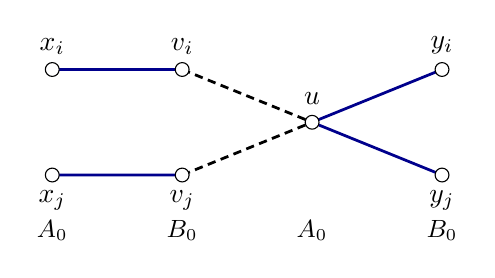
\begin{tikzpicture}[x=1.65cm,y=.67cm,
  vertex/.style={circle,draw,fill=white,inner sep=1.3pt,minimum size=5pt},
  reserve/.style={line width=1pt,blue!55!black},
  matched/.style={line width=1pt,densely dashed}]
  \coordinate (xi) at (0,1); \coordinate (xj) at (0,-1);
  \coordinate (vi) at (1,1); \coordinate (vj) at (1,-1);
  \coordinate (u) at (2,0);
  \coordinate (yi) at (3,1); \coordinate (yj) at (3,-1);
  \draw[reserve] (xi)--(vi) (xj)--(vj) (u)--(yi) (u)--(yj);
  \draw[matched] (vi)--(u) (vj)--(u);
  \foreach \name in {xi,xj,vi,vj,u,yi,yj} \node[vertex] at (\name) {};
  \foreach \name/\lab in {xi/x_i,vi/v_i,yi/y_i}
     \node[above=2pt] at (\name) {$\lab$};
  \foreach \name/\lab in {xj/x_j,vj/v_j,yj/y_j}
     \node[below=2pt] at (\name) {$\lab$};
  \node[above=3pt] at (u) {$u$};
  \foreach \col/\side in {0/$A_0$,1/$B_0$,2/$A_0$,3/$B_0$}
     \node[font=\small] at (\col,-2.05) {\side};
\end{tikzpicture}
\caption{Two colors can pass through the same left vertex \(u\). In color \(i\), the dashed edge \(v_i u\) belongs to the old matching, and the two solid edges are reserve copies. The lower walk makes the corresponding repair in color \(j\), using different reserve copies. Within a color, a second walk through the same matched vertex would reuse its old matching edge.}\label{fig:repair}
\end{figure}

\subsection{A factorization criterion using the nibble}

For the ordinary vertices, suppose the two physical sides each have size \(N\). Let \(C\) be a pool of ordinary crossing copies disjoint from the reserve \(R\). For specified free ordinary sets \(F_i,G_i\), the incidence hypergraph has one vertex for each left demand \((i,x)\) with \(x\in F_i\), one for each right demand \((i,y)\) with \(y\in G_i\), and one for each copy \(e\in C\). Each eligible use of a copy \(e=xy\) gives the triple
\[
 \{(i,x),(i,y),e\}.
\]
Eligibility requires \(x\in F_i\) and \(y\in G_i\). A demand degree counts eligible copies. A copy degree counts eligible colors. A codegree can exceed one only for two opposite demands in the same color, when there are parallel eligible copies between their endpoints.

We use the nibble estimate from Keevash~\cite[Section~3.1]{KeevashII}, in the equal-weight form derived from Ehard, Glock and Joos~\cite{EGJ}. Fix \(0<\delta<1\). For \(\Delta\) sufficiently large in terms of \(\delta\), let the incidence hypergraph have maximum degree at most \(\Delta\), codegrees at most \(\Delta^{1-\delta}\), and all demand degrees at least \((1-\eta)\Delta\), where \(0\le\eta<1\). If the number of triples and the number of tests are each at most \(\exp(\Delta^{(\delta/450)^2})\), there is a matching leaving uncovered mass at most
\[
 B(z)=\max\left\{(\eta+\Delta^{-\delta/450})z,\frac{3\Delta^\delta}{1-\eta}\right\}
 \label{eq:nibble-error}\tag{N}
\]
in every chosen test supported on demands, with weights in \([0,1]\) and total mass \(z\).

\begin{theorem}[Factorization from weighted reserves and a nibble]\label{thm:hybrid-completion}
Fix \(0<\delta<1\). Let \(M\) be a \(D\)-regular multigraph with a balanced cut and equally many ordinary vertices on each side. Its internal edges have a proper coloring with \(k\le D\) colors, leaving equally many free vertices on each side in every color.

Designate separate crossing copies for the exceptional rows in the two orientations, an ordinary pool \(C\), and a simple \(d\)-regular ordinary reserve \(R\), with \(d>0\). At each pair the sum of the designated copies is at most its multiplicity in \(M\). The two orientations of exceptional rows have the following weighted Hall certificates. For a row \(x\), let \(\eta_x\ge0\) be its charge per spent copy. Its weight at an ordinary column is between zero and \(\eta_x\) times the designated multiplicity at that pair. The total weight of a column is at most a common positive bound. In each color a free exceptional row has weight on the free ordinary columns at least that bound plus \((k-1)\eta_x\). The sufficient estimates \eqref{eq:rowx} and \eqref{eq:rowy} give such certificates when measured on the designated copies.

Suppose that after any feasible choice of exception-to-ordinary matchings covering all free exceptions and respecting their designated copies, the following conditions hold on the remaining free ordinary sets \(F_i,G_i\).
\begin{enumerate}
\item For some \(\Delta\) sufficiently large in terms of \(\delta\) and some \(0\le\eta<1\), the incidence hypergraph of \(C\) satisfies the degree and codegree bounds for \eqref{eq:nibble-error}. Both its number of triples and \(2N(k+1)\) are at most \(\exp(\Delta^{(\delta/450)^2})\).
\item The normalized matrix of \(R\) has norm at most \(\sigma<1\) on mean-zero vectors. Every physical vertex has at most \(\beta d\) reserve neighbors outside the opposite free set of any color. For an integer \(h\ge1\) with \(\sigma^h\le1/(2N)\), the quantities
\[
 \ell=2h+1,\qquad t=B(k),\qquad \rho=\beta+B(d)/d
\]
satisfy \eqref{eq:spectral-repair}.
\end{enumerate}
Then the \(k\) internal colors extend to perfect matchings with pairwise disjoint crossing copies, and \(M\) has a 1-factorization.
\end{theorem}

\begin{proof}
The weighted Hall argument from Theorem~\ref{thm:factor} covers the exceptional vertices. In each orientation, the at most \(k-1\) earlier colors can reduce a row's weight by at most \((k-1)\eta_x\). The remaining row and column bounds give Hall's inequality. The two orientations cover disjoint sets of vertices in each color because each joins an exception to an ordinary vertex. They remove the same number of vertices on each side of the cut, leaving \(|F_i|=|G_i|\).

We use two kinds of indicator tests for the nibble. For each physical vertex, we count its demands across the palette, with at most \(k\) demands. For each color and each physical vertex, we count the opposite free demands among its reserve neighbors, with at most \(d\) demands. There are \(2N(k+1)\) tests. The matching of triples gives initial matchings \(M_i\) in \(C\) with distinct physical copies across all the colors. The first tests bound the number of free missed sets containing any vertex by \(B(k)\). The second tests bound the number of newly missed ordinary neighbors by \(B(d)\) at each vertex in each color. Adding the previously unavailable neighbors gives the bound \(\beta d+B(d)=\rho d\) for the missed sets of Lemma~\ref{lem:spectral-repair}.

The lemma completes the ordinary matchings. Their copies and the copies used by the exceptional matchings fit the designated capacities at every physical pair. Together with the internal edges they give \(k\) disjoint perfect matchings. The residue has degree \(D-k\) and contains only crossing copies, so the regular bipartite residue factors by Hall's theorem.
\end{proof}

Hall's theorem supplies the exceptional matchings from the row and column bounds. The ordinary demand degrees and reserve neighborhoods depend on which vertices those matchings use. A bound on the losses that holds for every feasible matching therefore lets us apply the ordinary estimates to the choice supplied by Hall. If each side loses at most \(s\) ordinary vertices, each vertex of a simple pool loses at most \(s\) neighbors on the opposite side. Deleting eligible triples preserves the upper bounds on the copy degrees and codegrees. We use these bounds on the grid below.

\subsection{A sparse grid family outside the rectangle test}\label{sec:sparse-reserve-example}

Fix integers \(b\ge1\) and even \(q\ge12\). Each side has \(N=bq^2\) ordinary vertices on a \(q\)-by-\(q\) grid with \(b\) vertices per cell. We number rows and columns from \(0\) to \(q-1\). Two opposite vertices are adjacent in the grid support when they share a row or a column. Each support pair has one copy in \(C\) and another in \(R\), so both pools have degree \(d=b(2q-1)\). On cell-constant vectors the support matrix is \(b(J_q\otimes I_q+I_q\otimes J_q-I_{q^2})\), where \(J_q\) is the all-ones matrix. The eigenvalue on constants is \(d\). If exactly one coordinate function has sum zero, the eigenvalue is \(b(q-1)\). If both have sum zero, the eigenvalue is \(-b\). On vectors with sum zero in each cell the matrix is zero. Hence the normalized reserve has mean-zero norm \((q-1)/(2q-1)<1/2\).

We put \(d\) copies on one internal pair on the left and on one on the right. The pairs use columns \(0,1\) in row \(0\) on the left and in row \(q/2\) on the right. One copy of each pair goes into each of \(k=d\) colors. The internally free ordinary vertices are paired across the cut by equal coordinates wherever possible. The two remaining left coordinates in row \(q/2\) are paired with the two remaining right coordinates in row \(0\) in their respective columns. Each pair of this bijection receives \(d\) filler copies.

There are \(r=\lfloor\sqrt q\rfloor\) exceptions per side, paired across the cut. For each exceptional pair \(x,y\) we choose two distinct equal-coordinate filler pairs \(u_L,u_R\) in row \(q/2+1\), with the \(2r\) coordinates distinct across the exceptions. This is possible since \(2r\le q\). At either chosen coordinate the \(d\) filler copies are replaced by \(d\) copies each of \(u_Ly\) and \(xu_R\). We also put \(d\) copies on \(xy\). The replacements preserve each ordinary degree, which is \(3d\) from the two grid pools and the internal or filler copies. An exception has two ordinary neighbors of multiplicity \(d\) and its exceptional partner of multiplicity \(d\), so it too has degree \(3d\).

\paragraph{The hybrid parameters.}
Each exceptional row can assign weight \(d\) to its two ordinary neighbors, with column bound \(d\) and charge one. These neighbors are initially free in all colors and each column belongs to a single row in either orientation. After any feasible matching of the exceptions, each free ordinary side has size \(N-r-2\). A physical vertex loses at most \(r+2\) neighbors in either grid pool. Thus the incidence hypergraph has maximum degree at most \(d\), codegree at most one, and demand degrees at least \(d-r-2\). The number of triples is at most \(kNd\), and the number of tests is \(2N(k+1)\), both polynomial in \(q\).

We take \(\Delta=k=d\), \(\delta=1/4\), and \(\eta=\beta=(r+2)/d\). With \(b\) fixed, \(\eta=O(d^{-1/2})\), and
\[
 \frac{B(d)}{d}
 =\max\left\{\eta+d^{-1/1800},\,\frac{3d^{-3/4}}{1-\eta}\right\}
 =O(d^{-1/1800}).
\]
Thus \(t/d\) and \(\rho\) are both \(O(d^{-1/1800})\). Taking \(h=\lceil\log_2(2N)\rceil\) gives \(\ell=O(\log N)\). Since \(k=d\), the two left sides of \eqref{eq:spectral-repair} are bounded by \(O((\log N)^2d^{-1/1800})=o(1)\). This calculation gives the asymptotic application of Theorem~\ref{thm:hybrid-completion}.

\begin{corollary}[Grid factorization and rectangle separation]\label{cor:sparse-grid}
For every \(b\ge1\) and even \(q\ge12\), the multigraph just constructed has a 1-factorization. It has \(d=\Theta(\sqrt N)\) distinct ordinary crossing neighbors at each ordinary vertex and \(r=\Theta(N^{1/4})\) exceptions per side for fixed \(b\). The rectangle criterion of Theorem~\ref{thm:factor} fails for every admissible internal palette on this cut.
\end{corollary}

\begin{proof}
The explicit threshold comes from the filler pairs. In each of the \(d\) rounds we use one copy of each internal edge. At the first switched coordinate for \(x,y\), we match \(u_L\) to \(y\) and \(x\) to \(u_R\), using fresh copies in each round. The second switched coordinate for each pair of exceptions is still uncovered on both sides. Call it a hole. A hole can exchange its missing filler with any grid neighbor whose diagonal filler is intact. Excluding the four internal endpoint coordinates and all \(2r\) switched coordinates leaves at least \(d-(2r+4)\) choices at every hole.

We show that the exchanges can be scheduled whenever
\[
 r\le m_0=\left\lceil\frac d2\right\rceil
 \qquad\text{and}\qquad
 \left\lfloor\frac d2\right\rfloor\ge 2r+4.
\]
Each hole then has at least \(m_0\) eligible helpers. For each hole we select exactly \(m_0\) of them. This gives a simple bipartite graph of degree \(m_0\) at every hole and degree at most \(r\le m_0\) at every helper. By K\H{o}nig's bipartite edge-coloring theorem, these pairs split into \(m_0\) matchings. Every matching covers every hole, and the helpers used in a round are distinct. For \(q\ge12\), we have \(q\ge2r+5\). For \(r\le3\) this follows from \(q\ge12\), and for \(r\ge4\) it follows from \(q\ge r^2\). Since \(\lfloor d/2\rfloor\ge q-1\), both inequalities hold for every \(b\ge1\).

We duplicate the schedule, assigning the two occurrences to the two different grid pools, and keep \(d\) of the \(2m_0\) rounds. If a hole at coordinate \(z\) uses a helper at \(w\), its exchange uses \(z_Lw_R\) and \(w_Lz_R\). Both grid pairs exist because sharing a row or column is symmetric. The exchanges in a round are disjoint, and the pool and endpoint coordinates of a copy identify its hole, helper, and direction. Each hole uses a given helper at most once in each pool, so every copy used by an exchange is distinct. The unused helpers and the two off-diagonal filler pairs use separate copies of their fillers in each round. This gives \(d\) disjoint perfect matchings containing the internal copies. The residue is \(2d\)-regular and bipartite, so it factors.

For separation, let \(S\) be the left first half of the rows and \(T\) the right second half. They have total size \(N\). In either direction, a vertex of this rectangle sees \(bq/2\) vertices in the other half through its column and uses two grid copies at each. The filler copies on equal coordinates and the two fillers directed from the second half on the left to the first half on the right contribute zero to the rectangle. Thus every vertex has \(bq<d\) copies to the opposite set. A proper internal coloring needs at least \(d\) colors because each internal pair has \(d\) parallel copies. The rectangle exceeds the threshold \(N-r-2a\) of Theorem~\ref{thm:factor}, and its copies per vertex are fewer than the size of every admissible palette. The ordinary crossing support is exactly the grid support, since the off-diagonal fillers share a column. For fixed \(b\), the expressions for \(N,d,r\) give the stated growth rates.
\end{proof}

The grid separates the rectangle test from factorability on the specified cut. The explicit threshold \(q\ge12\) uses the filler matching to schedule deterministic exchanges. Theorem~\ref{thm:hybrid-completion} uses the bulk and reserve pools under the degree and spectral hypotheses, which hold for this grid for all sufficiently large \(q\) at fixed \(b\).


\section{Formalization}

The formalization companion~\cite{WECRCompanion} identifies the Lean proofs of the ten numbered results. They are checked in one Lean 4.35.0-rc3 project. The formal statement of Theorem~\ref{thm:hybrid-completion} includes an injective relabeling of the initial colors and proves that it preserves the color of each internal edge copy. The grid development checks both arguments in Section~\ref{sec:sparse-reserve-example}. The recoloring and cut proofs reuse the author's Overfull Criteria development~\cite{TraversoOverfull}. The companion points to the pinned dependencies, the verification logs, and the separate Certo calculation for Figure~\ref{fig:rectangle}.

\section*{Acknowledgments}

The author is deeply grateful to his wife María Paz and his children Lucas, Juan Cristóbal, Francisca, Raimundo and Benjamín for their love, patience and support.

\section*{Use of artificial intelligence and computational tools}

ChatGPT/Codex, by OpenAI, was used to explore and check arguments and to prepare the manuscript. Lean 4 and Mathlib were used for the proofs identified in the companion. The bipartite edge-coloring proof used to factor the residue comes from the formalization of the author's Erdős~81 Paper~V~\cite{TraversoV}, which credits Aristotle, by Harmonic, for the inherited Lean proofs.

Certo~\cite{Certo} produced the finite matrix certificate for the rectangular grid in Figure~\ref{fig:rectangle}. The companion points to the matrix specification, the certificate, and its verification report.

The author remains responsible for the arguments, citations, code, and presentation. No AI system is listed as an author.

\begin{thebibliography}{99}
\small

\bibitem{AB} G.~Ambrus and R.~Bozzai, Colorful vector balancing, \emph{Mathematika} \textbf{70} (2024), e12274. \href{https://doi.org/10.1112/mtk.12274}{doi:\,\nolinkurl{10.1112/mtk.12274}}.
\bibitem{Spencer} J.~Spencer, Balancing unit vectors, \emph{J. Combin. Theory Ser. A} \textbf{30} (1981), 349--350. \href{https://doi.org/10.1016/0097-3165(81)90033-9}{doi:\,\nolinkurl{10.1016/0097-3165(81)90033-9}}.
\bibitem{KLOS} D.~K\"uhn, A.~Lo, D.~Osthus and K.~Staden, The robust component structure of dense regular graphs and applications, \emph{Proc. Lond. Math. Soc.} \textbf{110} (2015), 19--56. \href{https://doi.org/10.1112/plms/pdu039}{doi:\,\nolinkurl{10.1112/plms/pdu039}}.
\bibitem{Haemers} W.~H. Haemers, Interlacing eigenvalues and graphs, \emph{Linear Algebra Appl.} \textbf{226--228} (1995), 593--616. \url{https://pure.uvt.nl/ws/files/996579/interlac.pdf}.
\bibitem{FFMYZ} A.~Ferber, B.~Frederickson, D.~Mao, L.~Yepremyan and Y.~Zhu, Regular bipartite decompositions of pseudorandom graphs, \emph{J. Combin. Theory Ser. B} \textbf{179} (2026), 270--292. \href{https://doi.org/10.1016/j.jctb.2026.04.004}{doi:\,\nolinkurl{10.1016/j.jctb.2026.04.004}}.


\bibitem{BKLS}
P.~N. Balister, A.~V. Kostochka, H.~Li and R.~H. Schelp,
Balanced edge colorings,
\emph{J. Combin. Theory Ser. B} \textbf{90} (2004), 3--20.
\href{https://doi.org/10.1016/S0095-8956(03)00073-X}{doi:\,\nolinkurl{10.1016/S0095-8956(03)00073-X}}.

\bibitem{CariolaroFu}
D.~Cariolaro and H.-L. Fu,
Covering graphs with matchings of fixed size,
\emph{Discrete Math.} \textbf{310} (2010), 276--287. \url{https://ir.lib.nycu.edu.tw/bitstream/11536/13011/1/000273169900010.pdf}.


\bibitem{CMS}
G.~Chen, J.~McDonald and S.~Shan,
Towards the Overfull Conjecture II,
preprint, 2026.
\href{https://arxiv.org/abs/2607.02270v1}{arXiv:2607.02270v1}.

\bibitem{Gale}
D. Gale, A theorem on flows in networks,
\emph{Pacific J. Math.} \textbf{7} (1957), 1073--1082.
\href{https://doi.org/10.2140/pjm.1957.7.1073}{doi:\,\nolinkurl{10.2140/pjm.1957.7.1073}}.

\bibitem{GK}
R.~Gajjala and A.~Khan,
Asymptotically Optimal Weighted Edge Colorings via Local Bin Packing,
preprint, 2026.
\href{https://arxiv.org/abs/2611.03190}{arXiv:2611.03190}.

\bibitem{McDiarmid}
C.~J.~H. McDiarmid,
The solution of a timetabling problem,
\emph{J. Inst. Math. Appl.} \textbf{9} (1972), 23--34.
\href{https://doi.org/10.1093/imamat/9.1.23}{doi:\,\nolinkurl{10.1093/imamat/9.1.23}}.

\bibitem{NashWilliams}
C.~St.~J.~A. Nash-Williams,
Amalgamations of almost regular edge-colourings of simple graphs,
\emph{J. Combin. Theory Ser. B} \textbf{43} (1987), 322--342. \url{https://www.sciencedirect.com/science/article/pii/0095895687900086}.


\bibitem{PlantholtShan}
M.~J. Plantholt and S.~Shan,
On the Multigraph Overfull Conjecture,
\emph{J. Graph Theory} \textbf{109} (2025), 226--236.
\href{https://doi.org/10.1002/jgt.23221}{doi:\,\nolinkurl{10.1002/jgt.23221}}.

\bibitem{Shan}
S.~Shan,
The overfull conjecture on graphs of odd order and large minimum degree,
\emph{J. Graph Theory} \textbf{106} (2024), 322--351. \href{https://doi.org/10.1002/jgt.23077}{doi:\,\nolinkurl{10.1002/jgt.23077}}.

\bibitem{SY}
A.~Shioura and M.~Yagiura,
A fast algorithm for computing a nearly equitable edge coloring with balanced conditions,
\emph{J. Graph Algorithms Appl.} \textbf{14} (2010), 391--407.
\href{https://doi.org/10.7155/jgaa.00213}{doi:\,\nolinkurl{10.7155/jgaa.00213}}.

\bibitem{BFU}
A.~Z. Broder, A.~M. Frieze and E.~Upfal,
Existence and construction of edge-disjoint paths on expander graphs,
\emph{SIAM J. Comput.} \textbf{23} (1994), 976--989.
\href{https://doi.org/10.1137/S0097539792232021}{doi:\,\nolinkurl{10.1137/S0097539792232021}}.

\bibitem{EGJ}
S.~Ehard, S.~Glock and F.~Joos,
Pseudorandom hypergraph matchings,
\emph{Combin. Probab. Comput.} \textbf{29} (2020), 868--885.
\href{https://arxiv.org/abs/1907.09946}{arXiv:1907.09946}.

\bibitem{KeevashII}
P.~Keevash, The existence of designs II,
preprint, 2018.
\href{https://arxiv.org/abs/1802.05900}{arXiv:1802.05900}.

\bibitem{EL}
P.~Erd\H{o}s and L.~Lov\'asz,
Problems and results on 3-chromatic hypergraphs and some related questions,
in \emph{Infinite and Finite Sets}, Colloq. Math. Soc. J\'anos Bolyai \textbf{10},
North-Holland, Amsterdam, 1975, 609--627.


\bibitem{Certo}
J.~P. Traverso Gianini, \emph{Certo: computational tools with verifiable certificates}, version 0.40.0. Commit \texttt{df0ec25178a6}. \url{https://github.com/jtraverso/certo-math}.

\bibitem{TraversoV}
J.~P. Traverso Gianini,
\emph{Colorability and realizability defects in resource-dominated packing relaxations}, Preprint 1.0, 2026.
\url{https://github.com/jtraverso/erdos-81-chordal-clique-partitions/tree/papers-v-vi-notes-preprint-1.0/preprints/PAPER_V}.

\bibitem{TraversoOverfull}
J.~P. Traverso Gianini, \emph{Overfull Criteria}, Lean 4 development.
Palomar record PALOMAR-2026-11-08-000004.
\url{https://github.com/jtraverso/overfull-criteria}.

\bibitem{WECRCompanion}
J.~P. Traverso Gianini,
\emph{Formalization companion to Weighted edge recoloring and 1-factorization across a cut}, Preprint 1.0, 2026.
\url{https://github.com/jtraverso/weighted-edge-recoloring/releases/download/preprint-1.0/WECR_FORMALIZATION_COMPANION_v1.0_en.pdf}.

\end{thebibliography}
\end{document}
